\chapter{Preliminaries}
\label{sec:preliminaries}

Before introducing the formal details of the new automaton model at the heart of this thesis, this chapter establishes the necessary theoretical foundation. We will review the standard definitions and notations from formal language theory, focusing on Deterministic Finite Automata (DFAs) as the canonical model for regular languages. Furthermore, we will define Deterministic Generalized Automata (DGAs), a key model for comparison that also utilizes strings on transitions but with a different matching rule. This groundwork will provide the vocabulary and context required to situate and analyze the suffix-reading paradigm presented in the chapters that follow.

\paragraph*{Basic notations.} We fix a finite alphabet $\Sigma$. Following standard convention, we
write $\Sigma^*$ for the set of all words (including $\e$) over
$\Sigma$, and $\Sigma^+ = \Sigma^* \setminus \{ \e\}$. For
$w \in \Sigma^*$, we write $|w|$ for the length of $w$, with $|\e|$
considered to be $0$.  A word $u$ is a \emph{prefix} of word $w$ if
$w = u v$ for some $v \in \Sigma^*$; it is a \emph{proper-prefix} if
$v \in \Sigma^+$. Observe that $\e$ is a prefix of every word. A set
of words $W$ is said to be a \emph{prefix-free set} if no word in $W$
is a prefix of another word in $W$. A word $u$ is a
\emph{suffix} (resp. \emph{proper-suffix}) of $w$ if $w = vu$ for some
$v \in \Sigma^*$ (resp. $v \in \Sigma^+$).

\begin{definition}[Deterministic Finite Automata (DFA)] \label{def:dfa}
A \emph{Deterministic Finite Automaton (DFA)} $M$ is a tuple
$(Q, \Sigma, q^{init}, \delta, F)$ where $Q$ is a finite set of
states, $q^{init} \in Q$ is the initial state, $F \incl Q$ is a set of
accepting states, and $\delta: Q \times \Sigma \to Q$ is a partial
function describing the transitions. If $\delta$ is complete, the
automaton is said to be a complete DFA. Else, it is called a trim
DFA. 
\end{definition}

The run of DFA $M$ on a word $w = a_1 a_2 \dots a_n$ (where
$a_i \in \Sigma$) is a sequence of transitions
$(q_0, a_1, q_1) (q_1, a_2, q_2) \dots (q_{n-1}, a_n, q_n)$ where $\delta(q_i, a_{i+1}) = q_{i+1}$ for each $0 \le i < n$, and
$q_0 = q^{init}$, the initial state of $M$. The run is accepting if
$q_n \in F$. If the DFA is complete, every word has a unique run. On a
trim DFA, each word either a has unique run, or it has no run. The
language $\Ll(M)$ of DFA $M$, is the set of words for which $M$ has an
accepting run.

\paragraph*{Nerode equivalence and minimality of DFAs.} 
We will now recall some useful facts about minimality of DFAs. Here,
by minimality, we mean DFAs with the least number of states. Every
complete DFA $M$ induces an equivalence $\sim_M$ over words:
$u \sim_M v$ if $M$ reaches the same state on reading both $u$ and $v$
from the initial state.  In the case of trim DFAs, this equivalence
can be restricted to set of prefixes of words in $\Ll(M)$. For a
regular language $L$, we have the Nerode equivalence: $u \approx_L v$
if for all $w \in \Sigma^*$, we have $uw \in L$ iff $v w \in L$. By
the well-known Myhill-Nerode theorem (see
\cite{DBLP:books/daglib/0016921} for more details), there is a
canonical DFA $M_L$ with the least number of states for $L$, and
$\sim_{M_L}$ equals the Nerode equivalence $\approx_L$. Furthermore,
every DFA $M$ for $L$ is a \emph{refinement} of $M_L$: $u \sim_M v$
implies $u \sim_{M_L} v$. If two words reach the same state in $M$,
they reach the same state in $M_L$.


\begin{definition}[Deterministic Generalized Automata (DGA)] \label{def:dga}
  A \emph{Deterministic Generalized Automaton (DGA)}~\cite{giammarresi1999deterministic} $H$ is given by
  $(Q, \Sigma, q^{init}, E, F)$ where $Q, q^{init}, F$ mean the same
  as in DFA, and $E \incl Q \times \Sigma^+ \times Q$ is a finite set
  of edges labeled with words from $\Sigma^+$. For every state $q$,
  the set $\{ \alpha \mid (q, \alpha, q') \in E \}$ is a prefix-free
  set.
\end{definition}
A run of DGA $H$ on a word $w$ is a sequence of edges
$(q_0, \alpha_1, q_1) (q_1, \alpha_2, q_2) \dots (q_{n-1}, \a_n, q_n)$
such that $w = \alpha_1 \alpha_2 \dots \a_n$, with $q_0$ being the
initial state. As usual, the run is accepting if $q_n \in F$. Due to
the property of the set of outgoing labels being a prefix-free set,
there is a atmost one run on every word. The language $\Ll(H)$ is the
set of words with an accepting run. Figure~\ref{fig:dfa-dga-examples}
gives examples of DFAs and corresponding DGAs.

\begin{figure}
  \centering
  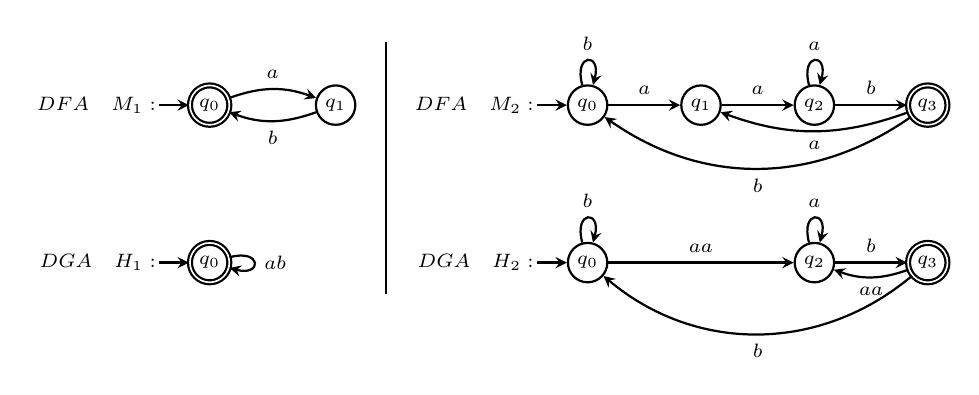
\begin{tikzpicture}[state/.style={circle, draw, thick, inner sep =
      2pt}, scale=0.8]
    \begin{scope}[every node/.style={state}]
      \node [double] (0) at (0,0) {\scriptsize $q_0$}; \node (1) at
      (2,0) {\scriptsize $q_1$};
    \end{scope}
    \begin{scope}[->,>=stealth, thick, auto]
      \draw (-0.8, 0) to (0); \draw (0) to [bend left=20] node
      {\scriptsize $a$} (1); \draw (1) to [bend left=20] node
      {\scriptsize $b$} (0);
    \end{scope}
    \node [left] at (-0.7, 0) {\scriptsize $DFA \quad M_1:$};

    \begin{scope}[yshift=-2.5cm]
      \begin{scope}[every node/.style={state}]
        \node [double] (0) at (0,0) {\scriptsize $q_0$};
      \end{scope}
      \begin{scope}[->,>=stealth, thick, auto]
        \draw (-0.8, 0) to (0); \draw (0) to [loop right] node
        {\scriptsize $ab$} (0);
      \end{scope}
      \node [left] at (-0.7, 0) {\scriptsize $DGA \quad H_1:$};
    \end{scope}

    \draw (2.8,-3) to (2.8,1);
    
    \begin{scope}[xshift = 6cm]
      \begin{scope}[every node/.style={state}]
        \node (0) at (0,0) {\scriptsize $q_0$}; \node (1) at (1.8,0)
        {\scriptsize $q_1$}; \node (2) at (3.6,0) {\scriptsize $q_2$};
        \node [double] (3) at (5.4,0) {\scriptsize $q_3$};
      \end{scope}

      \begin{scope}[->,>=stealth, thick, auto]
        \draw (-0.8, 0) to (0); \draw (0) to [loop above] node
        {\scriptsize $b$} (0); \draw (0) to node {\scriptsize $a$}
        (1); \draw (1) to node {\scriptsize $a$} (2); \draw (2) to
        [loop above] node {\scriptsize $a$} (2); \draw (2) to node
        {\scriptsize $b$} (3); \draw (3) to [bend left=20] node
        {\scriptsize $a$} (1); \draw (3) to [bend left=35] node
        {\scriptsize $b$} (0);
       
      \end{scope}
      \node [left] at (-0.7, 0) {\scriptsize $DFA \quad M_2:$};

      \begin{scope}[yshift=-2.5cm]
        \begin{scope}[every node/.style={state}]
          \node (0) at (0,0) {\scriptsize $q_0$}; \node (2) at (3.6,0)
          {\scriptsize $q_2$}; \node [double] (3) at (5.4,0)
          {\scriptsize $q_3$};
        \end{scope}
        \begin{scope}[->,>=stealth, thick, auto]
          \draw (-0.8, 0) to (0); \draw (0) to [loop above] node
          {\scriptsize $b$} (0); \draw (0) to node {\scriptsize $aa$}
          (2); \draw (2) to [loop above] node {\scriptsize $a$} (2);
          \draw (2) to node {\scriptsize $b$} (3); \draw (3) to [bend
          left=20] node {\scriptsize $aa$} (2); \draw (3) to [bend
          left=40] node {\scriptsize $b$} (0);
       
      \end{scope}
      \node [left] at (-0.7, 0) {\scriptsize $DGA \quad H_2:$};
    \end{scope}
  \end{scope}
 
\end{tikzpicture}
\caption{Examples of DFAs and corresponding DGAs, over alphabet
  $\{a, b\}$.}
\label{fig:dfa-dga-examples}
\end{figure}


It was
shown in~ \cite{giammarresi1999deterministic} that there is no unique smallest DGA. The paper defines an operation
to suppress states and create longer labels. A state of a DGA is
called \emph{superfluous} if it is neither the initial nor final state,
and it has no self-loop. For example, in
Figure~\ref{fig:dfa-dga-examples}, in $M_1$ and $M_2$, state $q_1$ is
superfluous. Such states can be removed, and every pair
$p \xra{\alpha} q$ and $q \xra{\beta} r$ can be replaced with
$p \xra{\alpha \beta} r$.  This operation is extended to a set of
states: given a DGA $H$, a set of states $S$, a DGA $\Ss(H, S)$ is
obtained by suppressing states of $S$, one after the other, in any
arbitrary order. For correctness, there should be no cycle in the
induced subgraph of $H$ restricted to $S$.
The paper proves that minimal DGAs (in number of
states) can be derived by suppressing states, starting from the
canonical DFA.



This chapter has provided the necessary formal preliminaries, defining the classical DFA model and the closely related DGA. With this foundational framework in place, we have established a common language and a basis for comparison. We are now prepared to move from these traditional prefix-matching models to the central contribution of this work. The following chapter will introduce the Deterministic Suffix-reading Automaton (DSA), presenting its formal syntax, its unique suffix-based operational semantics, and an initial analysis of its expressive power and succinctness.





%%% Local Variables:
%%% mode: latex
%%% TeX-master: "dsa-main"
%%% End:

